\documentclass[11pt,xcolor=dvipsnames,table]{beamer}
\usetheme{Szeged}
\usecolortheme{beaver}

\usepackage[utf8]{inputenc}
\usepackage[T1]{fontenc}
\usepackage[english]{babel}
\usepackage{amsmath}
\usepackage{amsfonts}
\usepackage{amssymb}
\usepackage{graphicx}
\usepackage{booktabs}
%\usepackage{tikz}
%\usetikzlibrary{calc,arrows,automata,shadows.blur,shapes,positioning,intersections}
\usepackage{hyperref}
\usepackage[absolute,overlay]{textpos}
%\usepackage[backend=biber, style=alphabetic, maxalphanames=1, sortlocale=en_US, natbib=true, url=false, doi=true, eprint=false, maxcitenames=1]{biblatex}
%\renewcommand*{\labelalphaothers}{}
\usepackage[algo2e]{algorithm2e}
\usepackage{caption}
\usepackage{subcaption}
\captionsetup{compatibility=false}
\usepackage{tabu}
\usepackage{multirow}
\usepackage{multicol}
%\addbibresource{References.bib}
%\bibliography{References}
%\renewcommand*{\bibfont}{\tiny} % resizes bibliography font size

\setbeamercolor{title}{fg=Brown,bg=Brown!20}
\setbeamercolor{frametitle}{fg=Brown,bg=Brown!20}
\setbeamercolor{section in head/foot}{bg=Brown}
\setbeamercolor{author in head/foot}{bg=Brown}
\setbeamercolor{date in head/foot}{fg=Brown}
\setbeamercolor*{item}{fg=Brown}


%\deftranslation[to=portuguese]{Theorem}{Teorema}
%\deftranslation[to=portuguese]{Proof}{Prova}

\defbeamertemplate*{footline}{shadow theme}
{%
	\leavevmode%
	\hbox{\begin{beamercolorbox}[wd=.5\paperwidth,ht=2.5ex,dp=1.125ex,leftskip=.3cm plus1fil,rightskip=.3cm]{author in head/foot}%
			\usebeamerfont{author in head/foot}\insertframenumber\,/\,\inserttotalframenumber\hfill\insertshortauthor
		\end{beamercolorbox}%
		\begin{beamercolorbox}[wd=.5\paperwidth,ht=2.5ex,dp=1.125ex,leftskip=.3cm,rightskip=.3cm plus1fil]{title in head/foot}%
			\usebeamerfont{title in head/foot}\insertshorttitle%
		\end{beamercolorbox}}%
		\vskip0pt%
	}

\AtBeginSection[]
{
	\begin{frame}{Index}
		\tableofcontents[currentsection, currentsubsection]
	\end{frame}
}

\AtBeginSubsection[]
{
	\begin{frame}{Index}
		\tableofcontents[currentsection, currentsubsection]
	\end{frame}
}

\author[Priscila Giovanella Vivian]{\textbf{Priscila Giovanella Vivian} \\ \vspace{10pt} {\scriptsize \textbf{Orientador: Prof. Dr. Rafael H. Bordini}}}
\title{Sistema de Cardápios Virtuais Acessível a Pessoas com Deficiência Visual}
%\subtitle{}
\logo{
\includegraphics[scale=0.35]{logo-pucrs.jpg}\hspace{1.05\linewidth}
\includegraphics[scale=0.35]{logo-facin.jpg}}
\institute[]{Pontifícia Universidade Católica do Rio Grande do Sul\\Faculdade de Informática\\Bacharelado em Sistemas de Informação}
\date{3 de julho de 2017}
%\subject{}
%\setbeamercovered{transparent}
%\setbeamertemplate{navigation symbols}{}

\begin{document}

	%%%%%%%%%%%%%%%%%%%%%%%%%%%%%%%%%%%%%%%%%%
	%%% TITLE PAGE %%%%%%%%%%%%%%%%%%%%%%%%%%%
	%%%%%%%%%%%%%%%%%%%%%%%%%%%%%%%%%%%%%%%%%%
	{
		\setbeamertemplate{headline}{}
		\setbeamertemplate{footline}{}
		\begin{frame}
			\titlepage
		\end{frame}
	}
	\addtocounter{framenumber}{-1} %desconta o primeiro slide da numeracao
	
	%%%%%%%%%%%%%%%%%%%%%%%%%%%%%%%%%%%%%%%%%%
	%%% INDEX %%%%%%%%%%%%%%%%%%%%%%%%%%%%%%%%
	%%%%%%%%%%%%%%%%%%%%%%%%%%%%%%%%%%%%%%%%%%
	\begin{frame}{Índice}
		\tableofcontents
	\end{frame}
	
	%%%%%%%%%%%%%%%%%%%%%%%%%%%%%%%%%%%%%%%%%%
	%%% MOTIVACAO %%%%%%%%%%%%%%%%%%%%%%%%%%%%
	%%%%%%%%%%%%%%%%%%%%%%%%%%%%%%%%%%%%%%%%%%
	\section{Motivação}\label{sec:intro}
\begin{frame}[allowframebreaks]{Motivação}
	\begin{itemize}
		\setlength{\itemsep}{0.5em}
		\item<1-> 18,7\% da população brasileira tem alguma deficiência visual.
		
		\item<1-> Brasileiros vêm migrando para os centros urbanos:
		\begin{itemize}
			\setlength{\itemsep}{0.5em}
			\item<1-> Recursos de acessibilidade em locais públicos ainda estão em processo de desenvolvimento;
			\item<1-> Pessoas deficientes visuais podem precisar de auxílio de tutores ou amigos em locais desconhecidos.
		\end{itemize}
		
		\item<1-> Em 2014, 136,6 milhões de brasileiros tinham aparelhos celulares:
			\begin{itemize}
				\item<1-> 49,4 milhões a mais que em 2008.
			\end{itemize}
	\end{itemize}
\end{frame}
	
	%%%%%%%%%%%%%%%%%%%%%%%%%%%%%%%%%%%%%%%%%%
	%%% OBJETIVOS %%%%%%%%%%%%%%%%%%%%%%%%%%%%
	%%%%%%%%%%%%%%%%%%%%%%%%%%%%%%%%%%%%%%%%%%
	\section{Objetivos}\label{sec:objetivos}
\begin{frame}{Objetivo Geral}
	Através de um cardápio digital desenvolvido para plataforma móvel, a pessoa com deficiência visual poderá ponderar sobre as opções fornecidas num determinado estabelecimento e, assim, decidir qual item do menu é de maior interesse, levando em consideração os diferentes tipos de alimentos, seus preços, sua disponibilidade, entre outros.
\end{frame}

\begin{frame}[allowframebreaks]{Objetivos Específicos}
	\begin{itemize}
		\setlength{\itemsep}{1em}
		\item<1-> Através do uso de uma ontologia, organizar os itens do menu em categorias
		\item<1-> Armazenar informações do usuário, como seus locais favoritos
		\item<1-> Armazenar informações sobre a quantidade de produtos disponíveis
		\framebreak
		\item<1-> Possibilitar o ordenamento do cardápio
			\begin{itemize}
				\setlength{\itemsep}{0.5em}
				\item<1-> Ordem alfabética
				\item<1-> Ordem de acesso
			\end{itemize}
		\item<1-> Permitir que a intereação com a aplicação seja acessível
		\item<1-> Desenvolver uma aplicação móvel que apresente os fatores listados acima
	\end{itemize}
\end{frame}
	
	%%%%%%%%%%%%%%%%%%%%%%%%%%%%%%%%%%%%%%%%%%
	%%% REFERENCIAL TEORICO %%%%%%%%%%%%%%%%%%
	%%%%%%%%%%%%%%%%%%%%%%%%%%%%%%%%%%%%%%%%%%
	\section{Referencial Teórico}\label{sec:referencial-teorico}
\begin{frame}{Ontologia}
	\begin{itemize}
		\setlength{\itemsep}{1em}
		\item<1-> Forma de especificar conceitos, objetos e relações numa área de interesse
		\item<1-> Propósito: compartilhamento e reutilização de conhecimento
		\item<1-> São muito utilizada na área de IA
		\item<1-> Difundiu-se na Internet, facilitando a busca e integração de informações
	\end{itemize}
\end{frame}

\begin{frame}{Criação de uma Ontologia}
	\begin{itemize}
		\setlength{\itemsep}{1em}
		\item<1-> Definir o domínio e escopo
		\item<1-> Listar termos considerados importantes
		\item<1-> Definir as classes e sua hierarquia
		\item<1-> Definir as propriedades das classes
	\end{itemize}
\end{frame}

\begin{frame}[allowframebreaks]{Acessibilidade, Ergonomia e Usabilidade}
	\begin{itemize}
		\setlength{\itemsep}{1em}
		\item<1-> Quatro princípios para o desenvolvimento de uma interface móvel acessível:
		\begin{itemize}
			\setlength{\itemsep}{0.5em}
			\item<1-> Perceptível
			\item<1-> Operável
			\item<1-> Compreensível
			\item<1-> Robusto
		\end{itemize}
		\item<1-> Não tentar replicar a experiência do computador de mesa
		\item<1-> Priorizar o conteúdo
		\framebreak
		\item<1-> Projetar para as diferentes orientações da tela
		\item<1-> Minimizar a carga de trabalho
		\item<1-> Minimizar a entrada de dados
		\item<1-> Adicionar textos descritivos aos controles como imagens, botões e campos de seleção
		\item<1-> Certificar-se que todos os campos de inserção ou toque possam ser acessados
		\framebreak
		\item<1-> Retornos multimodais
		\item<1-> Usar os controles já providos pelo sistema
		\item<1-> Evitar que controles desapareçam após um certo tempo
		\item<1-> Usar a ferramenta de \emph{dicas} em campos de texto editáveis
		\item<1-> Testar a aplicação com o TalkBack
	\end{itemize}
\end{frame}

\begin{frame}[allowframebreaks]{Trabalhos Relacionados}
	Tabelinha top.
\end{frame}
	
	%%%%%%%%%%%%%%%%%%%%%%%%%%%%%%%%%%%%%%%%%%
	%%% MODELAGEM %%%%%%%%%%%%%%%%%%%%%%%%%%%%
	%%%%%%%%%%%%%%%%%%%%%%%%%%%%%%%%%%%%%%%%%%
	\section{Modelagem}\label{sec:modelagem}
\begin{frame}[allowframebreaks]{Modelagem}
	\begin{itemize}
		\setlength{\itemsep}{0.5em}
		\item<1-> Metodologia Kanban
		\item<1-> Personas
		\item<1-> Histórias de Usuário:
		\begin{itemize}
			\setlength{\itemsep}{0.5em}
			\item<1-> US01 -- Acessar o sistema
			\item<1-> US02 -- Buscar restaurante
			\item<1-> US03 -- Acessar cardápio
			\item<1-> US04 -- Filtrar cardápio
			\item<1-> US05 -- Favoritar restaurante
		\end{itemize}
	\end{itemize}
\end{frame}

\begin{frame}[allowframebreaks]{Banco de Dados}
	\centering
	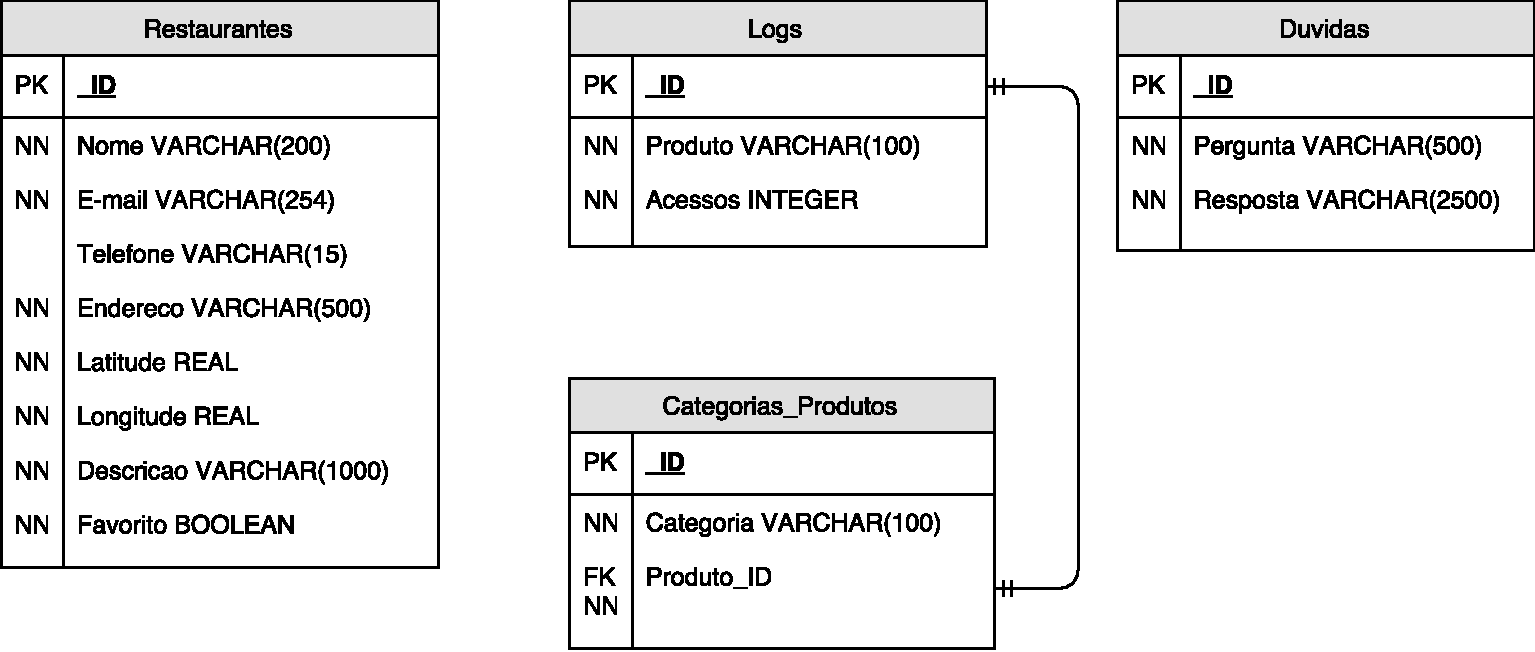
\includegraphics[width=1\linewidth]{../pdf/bd-slides.pdf}
\end{frame}

\begin{frame}{Fluxograma}
	\centering
	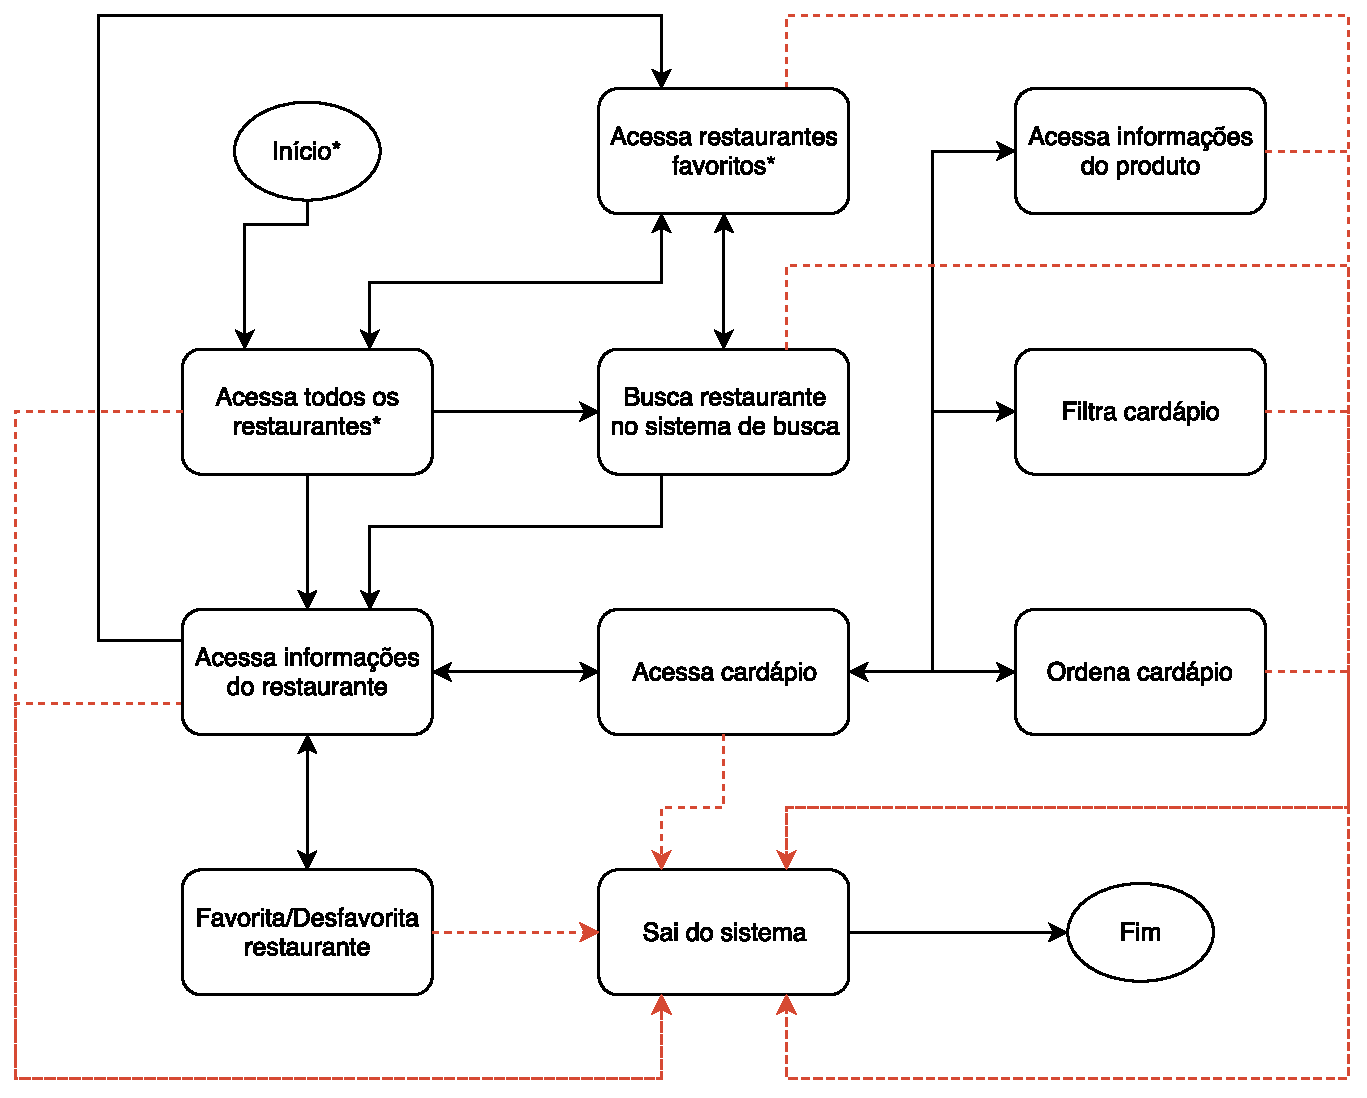
\includegraphics[width=0.8\linewidth]{../pdf/fluxograma-atual.pdf}
\end{frame}
	
	%%%%%%%%%%%%%%%%%%%%%%%%%%%%%%%%%%%%%%%%%%
	%%% DESENVOLVIMENTO %%%%%%%%%%%%%%%%%%%%%%
	%%%%%%%%%%%%%%%%%%%%%%%%%%%%%%%%%%%%%%%%%%
	\section{Desenvolvimento}\label{sec:desenvolvimento}
\begin{frame}[allowframebreaks]{Desenvolvimento}
	\begin{itemize}
		\setlength{\itemsep}{0.5em}
		\item :/
	\end{itemize}
\end{frame}
	
	%%%%%%%%%%%%%%%%%%%%%%%%%%%%%%%%%%%%%%%%%%
	%%% AVALIACAO %%%%%%%%%%%%%%%%%%%%%%%%%%%%
	%%%%%%%%%%%%%%%%%%%%%%%%%%%%%%%%%%%%%%%%%%
	\section{Avaliação}\label{sec:avaliacao}
\begin{frame}[allowframebreaks]{Avaliacao}
	\begin{itemize}
		\setlength{\itemsep}{0.5em}
		\item :/
	\end{itemize}	
\end{frame}
	
	%%%%%%%%%%%%%%%%%%%%%%%%%%%%%%%%%%%%%%%%%%
	%%% CONCLUSOES %%%%%%%%%%%%%%%%%%%%%%%%%%%
	%%%%%%%%%%%%%%%%%%%%%%%%%%%%%%%%%%%%%%%%%%
	\section{Conclusões}\label{sec:conclusoes}
\begin{frame}{Conclusões}
	\begin{itemize}
		\setlength{\itemsep}{1em}
		\item<1-> Dispositivos móveis oferecem recursos de acessibilidade a pessoas com deficiência visual, propiciando que as mesmas realizem atividades cotidianas
		\item<1-> Ferramentas de acessibilidade em dispositivos móveis (e.g., \emph{text-to-speech}) podem ser melhoradas
		\item<1-> O desenvolvimento da aplicação deve levar em consideração o \emph{feedback} dos usuários
		
	\end{itemize}
\end{frame}

\begin{frame}{Trabalhos Futuros}
	\begin{itemize}
		\setlength{\itemsep}{1em}
		\item<1-> Implementação das sugestões feitas pelas pessoas que avaliaram o sistema
		\item<1-> Recurso de \emph{login}
		\item<1-> Documentação e incrementação do sistema de ajuda
		\item<1-> Agente inteligente que faça sugestões aos usuários
		\item<1-> Integração com um \emph{cardápio inteligente}
	\end{itemize}
\end{frame}

	
	%%%%%%%%%%%%%%%%%%%%%%%%%%%%%%%%%%%%%%%%%%
	%%% QUESTIONS %%%%%%%%%%%%%%%%%%%%%%%%%%%%
	%%%%%%%%%%%%%%%%%%%%%%%%%%%%%%%%%%%%%%%%%%
	\begin{frame}
		\begin{center}
			{
				\LARGE
				Perguntas?	
			}
		\end{center}
	\end{frame}
	
	%%%%%%%%%%%%%%%%%%%%%%%%%%%%%%%%%%%%%%%%%%
	%%% BIBLIOGRAPHY %%%%%%%%%%%%%%%%%%%%%%%%%
	%%%%%%%%%%%%%%%%%%%%%%%%%%%%%%%%%%%%%%%%%%
%	\begin{frame}[allowframebreaks]
%		\printbibliography
%	\end{frame}
\end{document}